% !TEX program = xelatex
\documentclass[
  10pt,
  twoside,
  openany,
  b5paper, % 以上均为 ctexbook 提供的文类选项
  colorscheme = bootstrap-v4, % 请根据需要选择或定制配色方案
%  primary = blue,  % 主色
%  secondary = violet, % 辅助色
%  xits = false,
]{qyxf-book}


\title{Principles}
\subtitle{Notes on Statistical Mechanics: Theory and Molecular Simulation}  % 可选
\author{Xufan Gao}
\date{\today}
\typo{Xufan Gao}  % 排版人员信息,选填

% 定制元信息
\org{\Large\textit{浙江大学定量生物中心}\\\textsc{Institute of Quantitative Biology\\Zhejiang University}}
\footorg{\textsc{By Xufan Gao}}
\cover{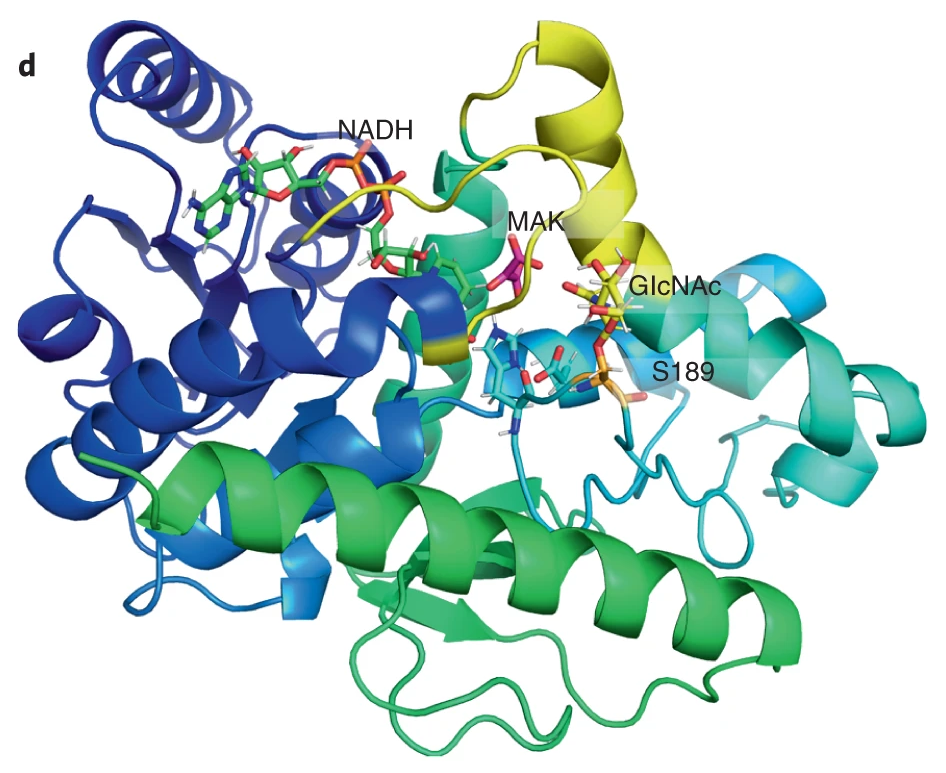
\includegraphics[width=.8\textwidth]{mdh.png}}
%\license{}  % 清空许可证信息

% 调整封面标题大小
\renewcommand{\titlefont}{\Huge\bfseries}
\renewcommand{\subtitlefont}{\LARGE\itshape}

% 取消本条注释,则将定义计数器归并到定理下
% \resetdefine

% customization
% English
%\usepackage[UTF8]{ctex}  % for rare Chinese comments
%\ctexset{today=old}
\usepackage{xeCJK}  % for rare Chinese comments
\linespread{1.2}  % together with xeCJK
\numberwithin{equation}{section}
\usepackage[version=4]{mhchem}

% 作品信息、环境名称是中文格式
\renewcommand{\chaptername}{Chapter\ }
\titleformat{\chapter}[block]{\color{\TitleColor}\centering\bfseries\fontsize{2.25em}{4.8ex}\selectfont\renewcommand{\arraystretch}{2}\linespread{2}}{\chaptername\thechapter}{1em}{}
\titleformat{\section}{\color{\TitleColor}\fontsize{1.75em}{2.5ex}\selectfont\bfseries\centering}{\S\,\thesection}{1em}{}
\renewcommand{\tablename}{Tab.}
\renewcommand{\figurename}{Fig.}
\renewcommand{\bibname}{References}
\renewcommand{\contentsname}{Table of Contents}
\setcounter{tocdepth}{1}

% user added math symbols
\newcommand{\md}{\mathrm{d}}
\newcommand{\der}[2]{\dfrac{\md #1}{\md #2}}
\newcommand{\dd}[2]{\dfrac{\md^2 #1}{\md #2^2}}
\newcommand{\p}[2]{\dfrac{\partial #1}{\partial #2}}
\newcommand{\pp}[2]{\dfrac{\partial^2 #1}{\partial #2^2}}
\newcommand{\pd}[3]{\dfrac{\partial^2 #1}{\partial #2 \partial #3}}
\newcommand{\vF}{\boldsymbol{F}}
\newcommand{\vr}{\boldsymbol{r}}
\newcommand{\vp}{\boldsymbol{p}}
\newcommand{\vq}{\boldsymbol{q}}
\newcommand{\vl}{\boldsymbol{l}}
\newcommand{\vx}{\boldsymbol{x}}
\newcommand{\dvr}{\dot{\vr}}
\newcommand{\ddvr}{\ddot{\vr}}
\newcommand{\dvq}{\dot{\vq}}
\newcommand{\dt}{\mathrm{d}t}
\newcommand{\half}{\dfrac{1}{2}}
\newcommand{\sumin}{\sum_{i=1}^N}
\newcommand{\suman}{\sum_{\alpha=1}^{3N}}
\newcommand{\lag}{\mathcal{L}} % Lagrangian
\newcommand{\ham}{\mathcal{H}} % Hamiltionian
\newcommand{\inttot}{\int_{t_1}^{t_2}}

\begin{document}

\maketitle


Oxford Graduate Texts

Tuckerman, M. E. (2010). Statistical mechanics: Theory and molecular simulation. Oxford: Oxford University Press.

As a freshman in college physics, there must be errors.

For normal examples, I won't number the equations.

\newpage
\tableofcontents

% !TeX root = demo.tex

\chapter{Classical Mechanics}

\section{Math recap}

\href{https://www.cnblogs.com/yanghh/p/13756471.html}{Link: take the derivative with respect to vectors}

\section{Newton's laws of motion}

Here we review some basic laws.

Newton's second law:
\begin{equation}
	\vF=m\dd{\vr}{t}=m\ddot{\vr} \label{eq:newton2nd}
\end{equation}

And Newton's third law:
\begin{equation}
	\vF_{AB}=-\vF_{BA}
\end{equation}

The definition of work:
\begin{equation}
	W_{AB}=\int_A^B\vF\cdot\md\vl
\end{equation}

In statistical mechanics, a particle $i$ will experience a force $\vF_i(\vr_1, \vr_2,\dots, \vr_N, \dot{\vr_i})$, which is determined by the positions of all other particles and its velocity. 

\section{Phase space: visualization}

We use position and momentum in the phase space because
\begin{equation}
	\vF=\der{\vp}{t} \label{rp}
\end{equation}

Phase space: $3N$ position variables and $3N$ momentum variables constitute the microscopic state of the system at time $t$, if the dimension is 3. These variables forms a so-called \textit{phase space vector} $x$. And by solving equations in the Newton's second law, we obtain a \textit{trajectory}:
\begin{equation}
	x_t=\left(\vr_1(t), \dots, \vr_N(t), \vp_1(t), \dots, \vp_N(t)\right) \label{eq:phase-space-vector}
\end{equation}

We can visualize the trajectory for a single one-dimensional particle. Some examples are (not explained here):
\begin{itemize}
	\item a free particle with momentum $p$.
	\item a harmonic oscillator, with an elliptical phase space.
	\item a particle crossing a "hill" potential
\end{itemize}

Visualizing a many-particle system is hard. Maybe we can consider a particular cut or surface representing a set of variables of interest, known as a \textit{Poincar{\'e} section}\footnote{庞加莱截面}.

\section{Lagrangian formulation of classical mechanics}

\vspace{0.5em}
\subsection{Conservative forces}
Conservative forces, means \textbf{energy conservation}. Defined as the negative gradient of $U$, the \textit{potential energy function}, Or for each particle $i$
\begin{tcolorbox}
	\begin{equation}
		\vF_i=-\nabla_i U(\vr_1,\dots,\vr_N) \label{eq:conservative}
	\end{equation}
\end{tcolorbox}
where $\nabla=\p{}{\vr}$. 

An important property is that, the work done by conservative forces only depends on the difference of $U$ of the start and end state, i.e. independent of the path taken. 
$$
%\oint\vF_i\md\vl=0
W_{AB}=U_B-U_A
$$

The kinetic energy of the system is given by
\begin{equation}
	K(\dvr_1, \dvr_2, \dots, \dvr_N)=\half\sum_{i=1}^{N}m_i\dvr_i^2 \label{eq:kinetics}
\end{equation}

\subsection{Formulation}
Here we introduce the \textit{Lagrangian} of a system
\begin{tcolorbox}
	\begin{equation}
		\lag=K(\dvr_1, \dots, \dvr_N)-U(\vr_1, \dots, \vr_N)
	\end{equation}
\end{tcolorbox}
which is the difference between the kinetic energy and potential energy. In contrast, the total energy is the sum of the two:
\begin{equation}
	E=K(\dvr_1, \dots, \dvr_N)+U(\vr_1, \dots, \vr_N)
\end{equation}

\begin{tcolorbox}[title={The Euler-Lagrange equation}]
	\begin{equation}
		\der{}{t}\p{\lag}{\dvr_i}=\p{\lag}{\vr_i} \label{eq:euler-lagrange}
	\end{equation}
	For any one of position coordinates, taking the partial derivative with respect to the velocity and then time, is equal to that with respect to the position directly.
\end{tcolorbox}
which can be verified with the substitution of eqn. \ref{eq:conservative} and \ref{eq:kinetics} (poco).

This equation helps generate the equations of motion. 

\example
Take the example of the one-dimensional harmonic oscillator, where
\begin{align*}
	U(x)&=\half kx^2\\
	K(\dot{x})&=\half m\dot{x}^2\\
	\der{}{t}\p{\lag}{\dot{x}}=\der{(m\dot{x})}{t}&=m\ddot{x}\\
	\p{\lag}{x}&=-kx
\end{align*}

It also helps to verify conservation of the energy.
\begin{align*}
	\der{E}{t}&=\sumin m\dvr_i\ddvr_i+\sumin\p{U}{\vr_i}\der{\vr_i}{t}\\
	&=\sumin m\dvr_i\ddvr_i-\sumin\vF_i\dvr_i\\
	&=\sumin m\dvr_i\ddvr_i-m\ddvr_i\dvr_i\\
	&=0
\end{align*}

\subsection{Generalized coordinates}
The power of Lagrangian formulation lies in the fact that the equations in an arbitrary coordinate system can be derived easily in order to address a particular problem. A set of $3N$ \textit{generalized coordinates} are related to the original Cartesian coordinate via
\begin{equation}
	q_\alpha = f_\alpha(\vr_1,\dots,\vr_N)\qquad \alpha=1,2,\dots,3N
\end{equation}
It is assumed that the transformation has a unique inverse
\begin{equation}
	\vr_i=\boldsymbol{g}_i(q_1,\dots,q_{3N})\qquad i=1,2,\dots,N
\end{equation}
Thus, through the chain rule, we have
\begin{equation}
	\dvr_i=\suman\p{\vr_i}{q_\alpha}\dot{q}_\alpha
\end{equation}

The kinetic energy can then be written as\footnote{separate everything containing $q$ ($i$) and the $\dot{q}$ velocities, by summing over $i$ first. Imagina a 3D cube, the z-axis is $m_i$, while on the x-y plane sits pairs of $q$ terms...}
\begin{align}\label{eq:kinetic-energy}
	K(\vq,\dvq)&=\half\sumin m_i\suman\p{\vr_i}{q_\alpha}\dot{q}_\alpha\sum_{\beta=1}^{3N}\p{\vr_i}{q_\beta}\dot{q}_\beta \notag\\
	&=\half\suman\sum_{\beta=1}^{3N}\sumin m_i\p{\vr_i}{q_\alpha}\p{\vr_i}{q_\beta}\dot{q}_\alpha\dot{q}_\beta \notag\\
	&=\half\suman\sum_{\beta=1}^{3N}G_{\alpha\beta}\dot{q}_\alpha\dot{q}_\beta
\end{align}
where
\begin{equation}
	G_{\alpha\beta}(\vq)=\sumin m_i\p{\vr_i}{q_\alpha}\cdot\p{\vr_i}{q_\beta}
\end{equation}
is the function of $q$ (so is $U(\vq)$). $\alpha$ and $\beta$ as indices, these elements forms a matrix $G$, the \textit{mass metric matrix}. 

Then the Lagrangian is expressed as a function of $\vq$ and $\dvq$. Adopting the Euler-Lagrange equation, considering $q_{\gamma}$ as $q_\alpha$:
\begin{equation}
	\der{}{t}\left(\sum_{\beta=1}^{3N}G_{\gamma\beta}\dot{q}_\beta\right)=\suman\sum_{\beta=1}^{3N}\p{G_{\alpha\beta}}{q_\gamma}\dot{q}_\alpha\dot{q}_\beta-\p{U}{q_\gamma} \label{eq:lag-equations}
\end{equation}
where $\gamma=1,\dots,3N$. These are the $3N$ equations of motion of the system.

\subsection{An example: two-particle system}
A two particle system subject to a potential $U$ which only depends on the distance between them. We can write:
\begin{equation}
	\lag=\half m_1\dvr_1^2+\half m_2\dvr_2^2-U(|\vr_1-\vr_2|) \label{eq:ex1.4}\\
\end{equation}
And knowing that (not important)
\begin{gather*}
	|\vr_1-\vr_2|=\sqrt{(x_1-x_2)^2+(y_1-y_2)^2+(z_1-z_2)^2}\\
	\p{|\vr_1-\vr_2|}{x_1}=\dfrac{2x_1}{2\sqrt{(x_1-x_2)^2+(y_1-y_2)^2+(z_1-z_2)^2}}=\dfrac{x_1}{|\vr_1-\vr_2|}\\
	\p{U(|\vr_1-\vr_2|)}{\vr_1}=\der{U(|\vr_1-\vr_2|)}{(|\vr_1-\vr_2|)}\p{|\vr_1-\vr_2|}{\vr_1}=\der{U(|\vr_1-\vr_2|)}{(|\vr_1-\vr_2|)}\dfrac{\vr_1}{|\vr_1-\vr_2|}\\
	\p{U(|\vr_1-\vr_2|)}{\vr_2}=-\der{U(|\vr_1-\vr_2|)}{(|\vr_1-\vr_2|)}\dfrac{\vr_2}{|\vr_1-\vr_2|}
\end{gather*}
, using eqn \ref{eq:euler-lagrange}, we can get
\begin{gather*}
	m_1\ddvr_1=-\der{U(|\vr_1-\vr_2|)}{(|\vr_1-\vr_2|)}\dfrac{\vr_1}{|\vr_1-\vr_2|}\\
	m_2\ddvr_2=\der{U(|\vr_1-\vr_2|)}{(|\vr_1-\vr_2|)}\dfrac{\vr_1}{|\vr_1-\vr_2|}
\end{gather*}

We now want to introduce a more natural set of general coordinates: \textit{center of mass} and \textit{relative position}:
\begin{gather*}
	\boldsymbol{R}=\dfrac{m_1\vr_1+m_2\vr_2}{m_1+m_2}\\
	\vr=\vr_1-\vr_2
\end{gather*}
Let $M=m_1+m_2$. The inverse of this transformation is
\begin{gather*}
	\vr_1=\boldsymbol{R}+\dfrac{m_2}{M}\vr\\
	\vr_2=\boldsymbol{R}-\dfrac{m_1}{M}\vr
\end{gather*}
Substituted into eqn \ref{eq:ex1.4}, the Lagrangian becomes
\begin{align*}
	\lag&=
	\half 
	m_1\left(\dot{\boldsymbol{R}}+\dfrac{m_2}{M}\dvr\right)^2+
	\half m_2\left(\dot{\boldsymbol{R}}-\dfrac{m_1}{M}\dvr\right)^2-U(|\vr|)\\
	&=\half M\dot{\boldsymbol{R}}^2+\half\mu\dvr^2-U(|\vr|)
\end{align*}
where \textit{reduced mass} $\mu=\dfrac{m_1m_2}{M}$.

Since the energy does not change as the center of mass moves, $\p{\lag}{\boldsymbol{R}}=0$. Then the equation of motion will be
\begin{gather*}
	M\ddot{\boldsymbol{R}}=0\\
	\mu\ddvr=-\der{U}{|\vr|}\dfrac{\vr}{|\vr|}
\end{gather*}
We can also transform $\vr$ further into spherical coordinates to obtain the one-dimensional equation of motion.

\section{Legendre transforms}

Consider a derivable function $f(x)$. Define
\begin{equation}
	s=f^\prime(x)=g(x)
\end{equation}
and assume $s=g(x)$ is a one-to-one mapping (i.e. $x=g^{-1}(s)$ exists).

For all $x=x_0$, 
\begin{equation*}
	f(x_0)=f^\prime(x_0)x_0+b(x_0)
\end{equation*}
holds, where $b(x_0)$ is the $y$-intercept. Thus, for all $x$
\begin{equation}
	f(x)=f^\prime(x)x+b(x)
\end{equation}

We now express the relation in the function of $s$, i.e. find the equivalent expression. Let $\tilde{f}=b$, then
\begin{equation}
	\tilde{f}=b(g^{-1}(s))=f(x(s))-sx(s)
\end{equation}
This is called a \textit{Legendre transform}\footnote{勒让德变换}.

For multiple variables $x_1, \dots, x_n$, there will be corresponding $s_1, \dots, s_n$, and the generalized form is
\begin{tcolorbox}
	\begin{equation}
		\tilde{f}(s_1, \dots, s_n)=f(x_1(s_1, \dots, s_n),\dots,x_n(s_1, \dots, s_n))-\sum_{i=1}^{n}s_ix_i(s_1, \dots, s_n)
	\end{equation}
	$f$ is constituted of $n$ pairs of variable $\times$ its derivative, plus a bias term $\tilde{f}$.
\end{tcolorbox}

\section{Hamiltonian formulation}

\vspace{1em}
\subsection{The Hamiltionian under Cartesian coordinates}

Before the derivation, An interesting fact is worth noting:
\begin{gather}
	\p{\lag}{\dvr_i}=\p{}{\dvr_i}\left[\sum_{i=1}\half m_i\dvr_i^2-U(\vr_i,\dots,\vr_N)\right]=m_i\dvr_i=\vp_i\\
	K=\sumin\half m_i\dvr_i^2=\half\sumin\vp_i\dvr_i\left(=\sumin\dfrac{\vp_i^2}{2m_i}\right)
\end{gather}
$\dvr_i$ is a function of $\vp_i$ ($\dvr_i(\vp_i)=\vp_i/m_i$; $s_i$ is $\vp_i$; $x_i$ is $\dvr_i$). 

The reason we introduce the Hamiltionian is to replace $\dvr_i$ in $\lag$ into $\vp_i$. Do the Legendre transform with $\vr_i$ fixed, plugging in the two equaitons above:
\begin{align}
	\tilde{\lag}&=\lag(\vr_1,\dots,\vr_N,\dvr_1(\vp_1),\dots,\dvr_N(\vp_N))-\sumin \vp_i\dvr_i(\vp_i) \notag\\
	&=\sumin\half \dfrac{\vp_i^2}{m_i}-U(\vr_1,\dots,\vr_N)-\sumin \dfrac{\vp_i^2}{m_i} \notag\\
	&=-\left(\sumin \dfrac{\vp_i^2}{2m_i}+U(\vr_1,\dots,\vr_N)\right)
\end{align}

Thus, the Hamilitonian is just the negative Legandre transformation of the Lagrangian:
\begin{tcolorbox}
	\begin{equation}
		\ham(\vr_1,\dots,\vr_N,\vp_1,\dots,\vp_N)=K(\vp_1,\dots,\vp_N)+U(\vr_1,\dots,\vr_N)
	\end{equation}
\end{tcolorbox}
which is the \textbf{total energy} of the system.

\subsection{Equations of motion under generalized coordinates}

Likewise, we can define the \textit{generalized momentum} $p_\alpha$ as
\begin{gather}
	p_\alpha=\p{\lag}{\dot{q}_\alpha} \label{eq:palpha}\\
	K(\vp,\dvq)=\half\suman p_\alpha\dot{q}_\alpha=\half\vp\cdot\dvq \label{eq:kinetic-general}
\end{gather}
for every set of generalized coordinates, where $\vp=(p_1,\dots,p_{3N})$ and $\dvq=(\dot{q}_1,\dots,\dot{q}_{3N})$.. These momenta are referred to as \textit{conjugated} to the coordinates. But why is there a $1/2$? Becuase $\dot{q}_\alpha$ is a function of $p_\alpha$.

Recall eqn \ref{eq:kinetic-energy}:
\begin{equation*}
	K=\half\suman\sum_{\beta=1}^{3N}G_{\alpha\beta}\dot{q}_\alpha\dot{q}_\beta
\end{equation*}
Comparing with eqn. \ref{eq:kinetic-general}, we can infer that
\begin{equation}
	p_\alpha=\sum_{\beta=1}^{3N}G_{\alpha\beta}\dot{q}_\beta
\end{equation}
In the form of matrix multiplication, it's $\vp=G\dvq$, or reversely
\begin{equation}
	\dvq=G^{-1}\vp
\end{equation}
which implies that $\dvq$ is a function of $\vp$. Though our mass metric matrix $G$ is a function of $\vq$, once the generalized coordinates are defined, $G$ remains unchanged. The value of $\vr$ and $\vq$ vary along the trajectory, but the direvatives do not.

For any set of generalized coordinates, the Hamiltionian is given similarly:
\begin{equation}
	\ham(\vq,\vp)=K(\vp,\dvq(\vp))+U(\vq) \label{eq:hamiltonian}
\end{equation}
where $K$ is only the function of $\vp$ ($m_i$ as constants) and $U$ is only the function of $\vq$.
%To be more specific,
%\begin{equation*}
%	K=\half\suman p_\alpha\dot{q}_\alpha=\half\vp^TG^{-1}\vp=\half\suman\sum_{\beta=1}^{3N}p_\alpha G^*_{\alpha\beta}p_\beta
%\end{equation*}
%where $G^{-1}(\alpha,\beta)=G^*_{\alpha\beta}$.

From eqn. \ref{eq:hamiltonian}, we can obtain by referring to eqn. \ref{eq:kinetic-general} and \ref{eq:conservative}:
\begin{tcolorbox}[title={Hamiltonian's equations of motion}]
	\begin{gather}
		\p{\ham}{p_\alpha}=\dot{q}_\alpha \qquad \p{\ham}{q_\alpha}=-\dot{p}_\alpha
		\label{eq:ham-equations}
	\end{gather}
	for $\alpha=1,\dots,3N$. 
\end{tcolorbox}

\example You may verify it in the example of harmonic oscillation:
\begin{gather*}
	\ham=\dfrac{p^2}{2m}+\half kx^2\\
	m\ddot{x}=\dot{p}=-\p{\ham}{x}=-kx
\end{gather*}

\mynote on the Hamiltonian equations of motion:
\begin{itemize}
	\item It's equivalent to Newton's second law of motion (eqn. \ref{eq:newton2nd}, with eqn. \ref{eq:palpha})
	\item It's equivalent to the Lagrangian equations of motion (eqn. \ref{eq:lag-equations}), which is a set of $3N$ second-order DEs. Eqn. \ref{eq:ham-equations} is a set of $6N$ first-order DEs and thus looks simpler.
\end{itemize}

\supplement I can't explain the $1/2$ yet...

\subsection{Properties}

\vspace{0.5em}
\subsubsection{Energy conservation}
\vspace{-1.2em}
\begin{align*}
	\der{\ham}{t}&=\suman \p{\ham}{q_\alpha}\dot{q}_\alpha+\p{\ham}{p_\alpha}\dot{p}_\alpha\\
	&=\suman\p{\ham}{q_\alpha}\p{\ham}{p_\alpha}+\p{\ham}{p_\alpha}(-\p{\ham}{q_\alpha})=0
\end{align*}

For a trajectory under constant energy, the phase space vectors (eqn. \ref{eq:phase-space-vector}) remain in a surface known as \textit{constant-energy (hyper)surface}.

\textit{Work-energy theroem} writes:
\begin{gather}
	K_A+U_A=K_B+U_B \notag\\
	U_B-U_A=W_{AB}=K_A-K_B
\end{gather}

Consider any arbitrary phase space function $a(x)$, a function of positions and momentums. We study its time evolution:
\begin{tcolorbox}
	\begin{align}
		\der{a}{t}&=\suman\p{a}{p_\alpha}\dot{p}_\alpha+\p{a}{q_\alpha}\dot{q}_\alpha \notag\\
		&=\suman\p{a}{p_\alpha}\p{\ham}{q}-\p{a}{q_\alpha}\p{\ham}{p_\alpha}\\
		&=\left\{a,\ham\right\} \label{eq:poisson-bracket}
	\end{align}
	where the last line is known as the \textit{Poisson bracket}.
\end{tcolorbox}

\example Suppose a system without external forces acting on it, which implies $\sumin \vF_i=0$, then consider the total momentum $\boldsymbol{P}=\sumin\vp_i$
\begin{align*}
	\left\{\boldsymbol{P},\ham\right\}&=\suman\left\{p_\alpha,\ham\right\}\\
	&=\suman\sum_{\beta=1}^{3N}\left[\der{p_\alpha}{r_\beta}\der{\ham}{p_\beta}-\der{p_\alpha}{p_\beta}\der{\ham}{r_\beta}\right] \qquad\text{($p$ and $q$ are independent)}\\
	&=\sum_{\beta=1}^{3N}\der{\ham}{r_\beta}=\sumin\der{\ham}{\vr_i}=\sumin\der{U}{\vr_i}=\sumin\vF_i=0
\end{align*}
which inplies that without external forces, the total momentum is conserved.

The Hamiltonian is invariant with respect to simply a translation transformation $\vr^\prime=\vr+\boldsymbol{a}$.

\subsubsection{Phase space incompressibility}
The derivative of the phase space vector $\vx$, $\eta$ is a function of $\vx$
\begin{gather}
	\dot{\vx}(t)=\left(\dot{q_1},\dots,\dot{q_{3N}},\dot{p_1},\dots,\dot{p_{3N}}\right) \notag\\
	\eta(\vx)=(\der{\ham}{p_1},\dots,\der{\ham}{p_{3N}},-\der{\ham}{q_1},\dots,\der{\ham}{q_{3N}}) \label{eq:etax}
\end{gather}

Divergence (散度) is defined as $\nabla_x=\p{}{\boldsymbol{x}}$, then
\begin{align*}
	\nabla_x\cdot\dot{\vx}&=\suman\p{\dot{q_\alpha}}{q\alpha}+\p{\dot{p_\alpha}}{p_\alpha}\\
	&=\suman\pd{\ham}{p_\alpha}{q_\alpha}+\pd{\ham}{(-q_\alpha)}{p_\alpha}=0
\end{align*}
which means there is no sources and sinks, called an incompressible flow in hydrodynamics.

\subsubsection{Symplectic structure}
As eqn. \ref{eq:etax} indicated
\begin{equation}
	\dot{\vx}=M\der{\ham}{\vx} \label{eq:xt}
\end{equation}
where $M$ is a matrix
\begin{equation}
	M=\begin{pmatrix}
		\boldsymbol{0} & \boldsymbol{I}\\
		-\boldsymbol{I}& \boldsymbol{0}
	\end{pmatrix}
\end{equation}
where $\boldsymbol{0}$ and $\boldsymbol{I}$ are $3N\times 3N$ zero and identity matrices respectively.

Consider a solution $\vx_t$ to eqn. \ref{eq:xt} starting from an initial condition $\vx_0$, $\vx_t$ is a unique function of $\vx_0$. This dependence can be viewed as a transformation from the beginning $6N$ variables to the end $6N$ variables\footnote{multivariate vector function, 多元向量值函数}, whose Jacobian matrix is
\begin{equation}
	J_{kl}=\p{x_t^k}{x_0^l}
\end{equation}
which is known as \textit{symplectic property}\footnote{辛性质}, and satisfies
\begin{tcolorbox}
	\begin{equation}
		M=J^TMJ
	\end{equation}
\end{tcolorbox}

\example the one-dimensional harmonic oscillator
\begin{gather*}
	x(t)=x_0\cos\omega t+\dfrac{p(0)}{m\omega}\sin\omega t\\
	p(t)=p_0\cos\omega t-m\omega x_0\sin\omega t
\end{gather*}
Thus, 
\begin{equation*}
	J=\begin{pmatrix}
		\cos\omega t & -m\omega\sin\omega t \\
		\dfrac{1}{m\omega}\sin\omega t & \cos\omega t
	\end{pmatrix}
\end{equation*}
and $M$ is just
\begin{equation*}
	\begin{pmatrix}
		0 & 1 \\
		-1 & 0
	\end{pmatrix}
\end{equation*}
then
\begin{align*}
	J^TMJ&=
	\begin{pmatrix}
		-\dfrac{1}{m\omega}\sin\omega t & \cos\omega t \\
		-\cos\omega t & -m\omega\sin\omega t
	\end{pmatrix}
	\begin{pmatrix}
		\cos\omega t & -m\omega\sin\omega t \\
		\dfrac{1}{m\omega}\sin\omega t & \cos\omega t
	\end{pmatrix}\\
	&=\begin{pmatrix}
		0 & 1 \\
		-1 & 0
	\end{pmatrix} = M
\end{align*}

\section{A simple classic polymer model}
变分法是处理泛函的数学领域,和处理函数的普通微积分相对。 譬如,这样的泛函可以通过未知函数的积分和它的导数来构造。 变分法最终寻求的是极值函数:它们使得泛函取得极大或极小值。 有些曲线上的经典问题采用这种形式表达:一个例子是最速降线,在重力作用下一个粒子沿着该路径可以在最短时间从点A到达不直接在它底下的一点B。

\section{The action integral}
\textit{The action integral} emerges naturally from quantum mechanics. It is defined as
\begin{tcolorbox}
	\begin{equation}
		A=\inttot\lag\left(\vq(t),\dvq(t)\right)\dt
	\end{equation}
\end{tcolorbox}
where $\vq=(q_1,\dots,q_{3N})$. $A$ is trajectory-dependent because it counts every value of $\vq$ and $\dvq$ from $t_1$ to $t_2$. Since a trajectory is a function of $t$, then the action integral is a \textit{functional}, usually denoted as $A\left[\vq\right]$.

\begin{tcolorbox}[colback=\TheoremBackground,colframe=\TheoremFrame,coltext=\TheoremColor]
	Definitions:
	\begin{itemize}
		\item A functional\footnote{泛函} is a quantity that depends on all values of a function between two points of its domain.
		\item A stationary point\footnote{驻点} is where the first order derivative of a function is zero.
		\item The variational principle\footnote{变分原理}. The variational method is to find an extremal function\footnote{极值函数} for a functional, just like to find an extreme value for a function.
	\end{itemize}
	A detailed introduction of the variational method is \href{https://zhuanlan.zhihu.com/p/139018146}{here}. A relevant example is to find the ground state wave function of a \ce{H2+}, where we use a linear combination of basis functions as the trial function, get the derivative of the total energy, let them equal to zero and calculate the coefficients. Then we obtain the wave function that may make the energy the lowest.
\end{tcolorbox}

Here we will do similar things to the action integral. 
First of all, such a trajectory must satisfy the endpoint conditions:
\begin{gather}
	\vq(t_1)=\vq_1,\qquad \dvq(t_1)=\dvq_1,\qquad \vq(t_2)=\vq_2,\qquad \dvq(t_2)=\dvq_2
\end{gather}

\begin{figure}[htbp]
	\centering
	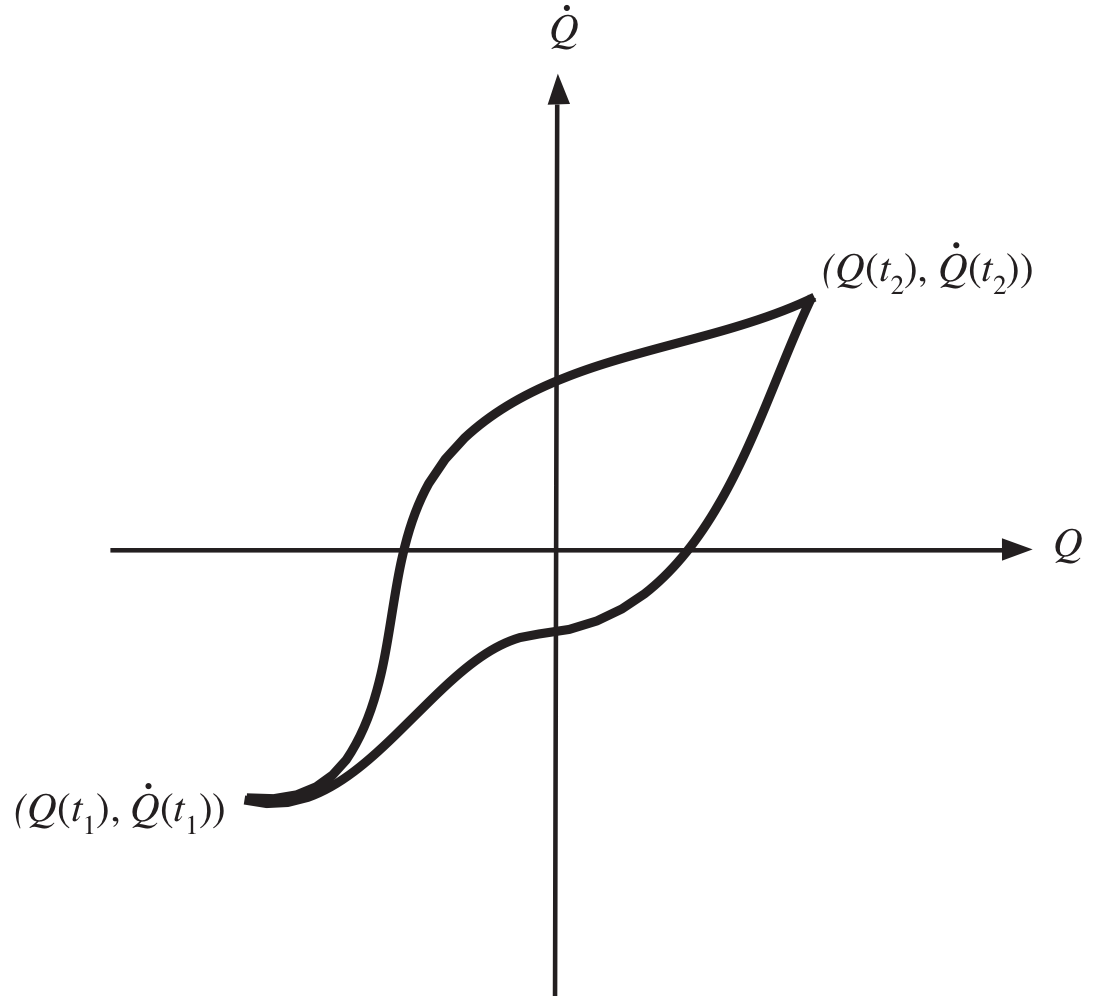
\includegraphics[width=0.6\linewidth]{figure/1.8-qt}
	\caption{Two proposed paths joining the fixed endpoints.}
	\label{fig:1.8-qt}
\end{figure}

Second, for a slightly changed trajectory $\vq(t)+\delta \vq(t)$ that also satisfies the endpoint conditions, i.e.
\begin{gather}
	\delta\vq(t_1)=\delta\vq(t_2)=0,\qquad \delta\dvq(t_1)=\delta\dvq(t_2)=0
\end{gather}
where $\delta\vq$ is called the variation of $\vq$\footnote{$\delta\vq$是$\vq$的变分},
the variation of $A$ must be zero, which means
\begin{equation*}
	\delta A=\inttot\lag\left(\vq(t)+\delta\vq(t),\dvq(t)+\delta\dvq(t)\right)\dt
	-\inttot\lag\left(\vq(t),\dvq(t)\right)\dt=0
\end{equation*}
Perform a first-order Taylor expansion to the first term, we get
\begin{equation*}
	\delta A=\inttot\left[\p{\lag}{\vq(t)}\delta\vq(t)+\p{\lag}{\dvq}\delta\dvq(t)\right]\dt
\end{equation*}
Knowing that $\delta\dvq(t)=\der{\left[\delta\vq(t)\right]}{t}$, and hoping to merge the two $\delta$ terms, we integrate the second term by parts\footnote{integrate ... by parts: 分部积分法}
\begin{align}
	\delta A&=\inttot\p{\lag}{\vq(t)}\delta\vq(t)\dt+\p{\lag}{\dvq}\md\left[\delta\vq(t)\right] \notag\\
	&=\left.\p{\lag}{\dvq}\delta\vq(t)\right|_{t_1}^{t_2}+\inttot\left[\p{\lag}{\vq(t)}-\der{}{t}\left(\p{\lag}{\dvq(t)}\right)\right]\delta\vq(t)\dt=0 \label{eq:deltaA}
\end{align}
Since $\delta\vq(t)=0$ at $t_1$ and $t_2$, the first term is 0; for any $\delta\vq$ the above equation holds, then there must be
\begin{equation}
	\p{\lag}{\vq}-\der{}{t}\left(\p{\lag}{\dvq}\right)=0
\end{equation}
or 
\begin{equation}
	\der{}{t}\left(\p{\lag}{\dot{q}_\alpha}\right)-\suman\p{\lag}{q_\alpha}=0
\end{equation}
which is exactly the Euler-Lagrange equation (eqn. \ref{eq:euler-lagrange}).

In statistical mechanics, we care more about endpoint problems than initial-value problems, though the solution to the "endpoint problem"\footnote{相比于初值问题,有两个条件要满足} is not guaranteed to be a "stationary function". We are interested in the behaviors of large numbers of trajectories all seeded differently. Initial conditions for Hamilton's equations are generally chosen at random (e.g. random velocities). And we are interested in paths that evolve from one region of phase space to another, but not one point to another.

\section{Lagrangian mechanics and systems with constraints}
It is often necessary to impose constraints to a system.

\example \begin{itemize}
	\item high-frequency (rigid) chemical bonds
	\item thermal or barostatic control mechanisms
\end{itemize}

A system with $N_c$ constraints have $3N-N_c$ degrees of freedom, and must satisfy $N_c$ equations of the coordinates and velocities.

\textit{Holonomic constraints}\footnote{完整约束,相对地有非完整约束}: all relationships are functions of only the coordinates and time:
\begin{equation}
	\sigma_k(q_1,\dots,q_{3N},t)=0\quad \text{for } k=1,2,\dots,N_c
\end{equation}
If not, the constraints are said to be \textit{nonholonomic constraints}. 
For example, to keep the kinetic energy (temperature) constant, the system must satisfy
\begin{equation}
	\sumin\half m_i\dvr_i^2-C=0 \label{eq:kinetic-constrain}
\end{equation}
where $C$ is a constant.

Constraints will reduce the degrees of freedom, which is good, but it is not always convienent to write new equations particularly when there is a large number of coupled constraints. 
Then we try to incorporate them into the framework of classical mechanics.
We apply the method of \textit{Lagrangian undetermined multiplier}\footnote{拉格朗日待定乘子}, but the constraint conditions of a trajectory $\vq(t)$ must satisfy
\begin{tcolorbox}
	\begin{equation}
		\suman a_{k\alpha}\md q_\alpha+a_{kt}\md t=0 \label{eq:lag-multiplier}
	\end{equation}
\end{tcolorbox}
where $a_{k\alpha}$ is a set of coefficients for the displacements $\md q_\alpha$. For a holonomic constraint, they can be obtained by
\begin{gather}
	a_{k\alpha}=\p{\sigma_k}{q_\alpha}\\
	a_{kt}=\p{\sigma_k}{t}
\end{gather}
In other words, $\md\sigma_k$ is an exact differential\footnote{全微分,也称perfect differential} of $q_\alpha$ and $t$. Eqn. \ref{eq:lag-multiplier} can be easily derived from $\md\sigma_k=0$.

Similarly, we can obtain the variation of $\sigma_k$\footnote{Please refer to \href{https://www.bilibili.com/video/BV1xJ411s78q?p=59}{this fantastic MOOC}, which told me the differentiation and variation of a variable are similar in form (perfect differential), while the latter assumes time does not change. We can write both $\md q$ and $\delta q$.}
\begin{equation}
	\delta\sigma_k=\suman a_{k\alpha}\delta q_\alpha=0
\end{equation}
where $t$ is not included in the variation form.

\mynote The original text: Assuming that the constraints can be expressed in the differential form of eqn. \ref{eq:lag-multiplier}, we must also be able to express them in terms of path displacements $\delta q_\alpha$ in order to incorporate them into the action principle. Unfortunately, doing so requires a further restriction, since it is not possible to guarantee that a perturbed path $Q(t) + \delta Q(t)$ satisfies the constraints. The latter will hold if the \textbf{constraints are integrable}, in which case they are expressible in terms of path displacements as eqn. \ref{eq:lag-multiplier}.

\supplement My comprehesion. If $\vq(t)$ satisfies $\sigma_k$, then $\vq(t)+\delta\vq(t)$, with only a slight change, will also also satisfy $\sigma_k$. But only $\vq$ is changed/in $\delta \vq(t)$ ($\dvq$ is not), so $\sigma_k$ should only contain $\vq$ and $t$?

In contrast, nonholonomic constraints can not always be expressed in the form of eqn. \ref{eq:lag-multiplier}, but a notable exception is eqn. \ref{eq:kinetic-constrain}
\begin{gather*}
	\sumin\half m_i\dvr_i^2-C=0\\
	\sumin\half m_i\dvr\md\vr_i-C\dt=0
\end{gather*}
where $a_{ki}=\half m_i\dvr$.

We then add eqn. \ref{eq:lag-multiplier} as Lagrange undetermined multipliers into eqn. \ref{eq:deltaA}:
\begin{equation}
	\delta A=\inttot\left[\suman\p{\lag}{q_\alpha(t)}-\suman\der{}{t}\left(\p{\lag}{\dot{q}_\alpha(t)}\right)+\sum_{k=1}^{N_c}\suman \lambda_ka_{k\alpha}\right]\delta\vq(t)\dt
\end{equation}
Thus, the new equations of motion can be derived from $\delta A=0$:
\begin{tcolorbox}
	\begin{equation}
		\der{}{t}\left(\p{\lag}{\dot{q}_\alpha(t)}\right)-\p{\lag}{q_\alpha(t)}=\sum_{k=1}^{N_c}\lambda_ka_{k\alpha} \qquad \text{for}\ \alpha=1,\dots,3N
		\label{eq:motion-cons}
	\end{equation}
\end{tcolorbox}
this equation holds for every $\alpha$ because every $\delta q$ is independent of each other.

Also, eqn. \ref{eq:lag-multiplier} can be written as
\begin{equation}
	\suman a_{k\alpha}\dot{q}_\alpha+a_{kt}=0
	\qquad \text{for}\ k=1,\dots,N_c
	\label{eq:cons-time}
\end{equation}
Eqns. \ref{eq:motion-cons} together with eqns. \ref{eq:cons-time} constitute a set of $3N+N_c$ equations for $3N+N_c$ variables ($q_\alpha, \lambda_k$)?

Still for holonomic constraints,
\begin{equation}
	\ham=U+K+\sum_{k=1}^{N_c}\lambda_k\sigma_k
\end{equation}

where




\supplement 自己的一点理解,不知道对不对

\begin{itemize}
	\item 完整约束:(积分后)与速度无关。如物体只能在静止的面上运动。
	\item 稳定约束:约束不随时间变化。如物体只能在固定平面上运动。
	\item 理想约束:约束力做的虚功为零。如物体只能在光滑水平面上运动。
\end{itemize}

虚位移是某一时刻对$\vr$加一个微扰,位移的变分是对整个时间段$t_1\sim t_2$加一个微扰,不一样但都是虚拟微扰。

虚功原理,分析力学下的平衡条件:主动力虚功为零。对应、等价于牛顿第一、二定律。


\section{Gauss's principle of least constraint}

\begin{equation}
	m\dot{\dot{\vr}}=\vF(\vr)+\lambda\nabla\sigma
\end{equation}

\section{Rigid body motion}
We may treat small molecules or groups as a \textit{rigid body}, i.e. fixing the bond length, angles (or for example, the distance between the two hydrogen atoms in a water molecule), etc.


\section{Non-Hamiltonian systems}


\section{Problems}


\section*{Summary of chapter}

\begin{itemize}
	\item Phase space vector: $3N$ position and $3N$ momentum variables.
	\item Euler-Lagrange equation: \[ \der{}{t}\p{\lag}{\vr}=\p{\lag}{\dvr} \]
	\item the Hamiltonian ($\ham=-(K+U)=-E$) is a Legendre transform of the Lagrangian ($\lag=K-U$).
	\item 
\end{itemize}
\chapter{Theoretical of foundations of classical statistical mechanics}

\section{Overview}

It's statistical mechanics' job to communicate between macroscopic thermodynamics and microscopic laws of motion. Thermodynamics is a phenomenological theory which makes no reference to the microscopic constituents of matter; however, we can rationalize thermodynamics based on microscopic mechanical laws illustrated in chapter 1. But problems emerge:
\begin{itemize}
	\item marcoscopic systems possess an enormous number of degree of freedom, or number of particles;
	\item in real-world systems, the interactions between particles are highly nontrivial;
	\item microscopic mechanical laws are "inherently reversible", while the second law of thermodynamics prescribes a direction of time, which is known as \textit{Loschmidt's paradox}.
\end{itemize}
People then realized that macroscopic properties of a system do not depend strongly on the motion of every particle, but rather on gross averages that "wash out" microscopic details. 

The principal conceptual breakthough is that of an \textit{ensemble}, which refers to a collection of systems that share common macroscopic properties. This chapter is mainly about this genius idea.

\section{The laws of thermodynamics}



\section{Overview}

\section{Overview}


\section*{Summary of chapter}

\begin{itemize}
	\item 
	\item 
\end{itemize}


% !TeX root = demo.tex

\chapter{内容示例}
\section{用户环境示例}

\begin{tcolorbox}
	\begin{description}
		\item [GRE备考指南] \url{https://qyxf.site/latest/GRE备考指南-v2.0.pdf}
		\item [军事理论教程] \url{https://qyxf.site/latest/军事理论教程.pdf}
		\item [分析力学笔记] \url{https://qyxf.site/latest/分析力学笔记-v1.0.pdf}
		\item [大学物理题解] \url{https://qyxf.site/latest/大物题解(上).pdf}
		\item [实变函数习题解答] \url{https://qyxf.site/latest/实变函数习题解答.pdf}
		\item [计算方法撷英] \url{https://qyxf.site/latest/计算方法撷英-v1.1.pdf}
		\item [计算机程序设计指南] \url{https://qyxf.site/latest/计算机设计程序指南.pdf}
	\end{description}
\end{tcolorbox}

\begin{pequation}
	\textit{Euler-Lagrangian equation}
	$$
	\dd{}{t}\p{\lag}{\dvr_i}=
	$$
\end{pequation}

\begin{define}
	极限就是超越自我。
\end{define}

\begin{theorem}
	任何极限都可以直接观察得出。
\end{theorem}

\begin{lemma}
	以上内容,纯属扯淡。
\end{lemma}

\begin{corollary}
	这是一个推论。
\end{corollary}

\begin{note}
	好好学习,天天向上。
\end{note}

\begin{alert}
	今天你学习了吗?
\end{alert}

\section{列表样式}
\begin{itemize}
	\item 这是第一层
	\item 这也是第一层
	\begin{itemize}
		\item 这是第二层
		\begin{itemize}
			\item 这是第三层
		\end{itemize}
	\end{itemize}
\end{itemize}

\begin{enumerate}
	\item 这是第一层
	\item 这也是第一层
	\begin{enumerate}
		\item 这是第二层
		\begin{enumerate}
			\item 这是第三层
		\end{enumerate}
	\end{enumerate}
\end{enumerate}

\section{正文示例}

\textbf{微分学}(\emph{differential calculus})是微积分的一部分,是通过\emph{导数}和\emph{微分}来研究曲线斜率、加速度、最大值和最小值的一门学科,也是探讨特定数量变化速率的学科。微分学是微积分的两个主要分支之一,另一个分支则是\textbf{积分学},探讨曲线下的面积。


\begin{table}[htbp]
	\centering
	\caption{常用导数}
	\begin{tabular}{cccc}
		\toprule
		\textbf{原函数} & \textbf{导函数}   & \textbf{原函数} & \textbf{导函数} \\
		\midrule
		$C$             & $0$               & $\ln x$         & $\frac{1}{x}$   \\
		$x^\mu$         & $\mu x^{\mu - 1}$ & $\sin x$        & $\cos x$        \\
		$e^x$           & $e^x$             & $\cos x$        & $-\sin x$       \\
		\bottomrule
	\end{tabular}
\end{table}

……几乎所有量化的学科中都有\textbf{微分}的应用。例如在物理学中,运动物体其\emph{位移}对时间的导数即为其\emph{速度},\emph{速度}对时间的导数就是\emph{加速度}、物体\emph{动量}对时间的导数即为物体所受的\emph{力},重新整理后可以得到牛顿第二运动定律 $F=ma$ 。化学反应的\emph{化学反应速率}也是导数。在运筹学中,会透过导数决定在运输或是设计上最有效率的做法。

\begin{figure}[htbp]
	\centering
	
\includegraphics[width=.3\textwidth]{qyxf-cover.pdf}
	\caption{V2 版本的封面图片}
	\label{fig:qyxf-logo}
\end{figure}

导数常用来找函数的\emph{极值}。含有微分项的方程式称为\textbf{微分方程},是自然现象描述的基础。微分以及其广义概念出现在许多数学领域中,例如\emph{复分析}、\emph{泛函分析}、\emph{微分几何}、\emph{测度}及\emph{抽象代数}\footnote{以上内容摘自维基百科中文词条 --- 微分学:\url{https://zh.wikipedia.org/wiki/微分学}。}。

\section{引导命令示例}

\exercise{1} 试用配方法求解方程:
\begin{equation}\label{eq:quadratic}
	ax^2 + bx + c = 0
\end{equation}

\solve 首先,方程左右两侧同除以 $a$,得到
\[ x^2 + \frac bax + \frac ca = 0 \]
根据一次项来配方,按公式 $(x+A)^2=x^2+2Ax+A^2$ 配出常数项:
\[ x^2 + \frac bax + \left(\frac b{2a}\right)^2 + \frac ca - \left(\frac b{2a}\right)^2 = 0 \]
配方并移项得到
\[ \left(x + \frac b{2a}\right)^2 = \frac {b^2}{4a^2} - \frac ca \]
方程左右开方,得
\[ x + \frac b{2a} = \pm \sqrt{\frac {b^2}{4a^2} - \frac ca} \]
从而得到方程 \eqref{eq:quadratic} 之解为
\begin{equation}
	x = - \frac b{2a} \pm \sqrt{\frac {b^2}{4a^2} - \frac ca}
\end{equation}
该式即为一元二次方程的\textbf{通用求根公式}。


\analysis 在这一问题中,需要注意以下几点 \cite{texbook,latex}:
\begin{itemize}
	\item ……
	\item ……
	\item ……
\end{itemize}

%\begin{thebibliography}{99}
%  \bibitem{texbook} KNUTH~D~E. The \TeX book [M]. Addison-Wesley: Reading, 1986.
%  \bibitem{latex} 刘海洋. \LaTeX 入门 [M]. 人民邮电出版社: 北京, 2013.
%\end{thebibliography}








\end{document}